\begin{frame}[t]{Returnees: did they come back to the same position?}
    \hypertarget{app:postwar-position-return}{}
    \centering
    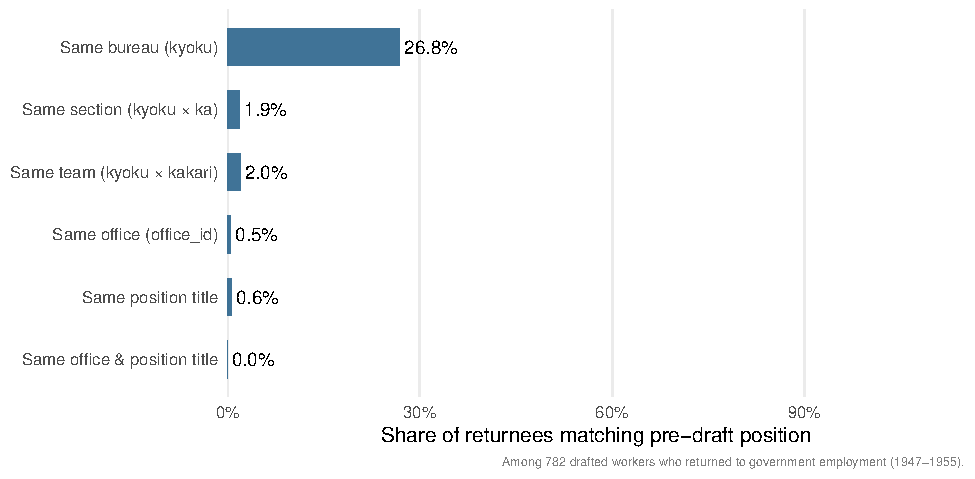
\includegraphics[width=0.84\textwidth]{Results/drafted_postwar_return/positional_match_rates.pdf}
    \vspace{1mm}
    \parbox{0.9\textwidth}{\centering\tiny Among the 782 drafted workers who returned to Tokyo metropolitan government employment (1947--1955), the figure shows what share returned to the same organizational unit at each level of the hierarchy. Only 26.8\% returned to the same bureau; virtually none (0.5\%) returned to the same office. The 1943 Tokyo Fu/Shi merger and postwar reorganization largely dissolved the original structure.}
\end{frame}

\begin{frame}[t]{Same-bureau return and postwar tenure}
    \scriptsize
    \centering
    \begin{threeparttable}
    \begin{tabular}{lcc}
        \toprule
        & \multicolumn{2}{c}{Postwar years observed} \\
        \cmidrule(lr){2-3}
        & (1) No FE & (2) Bureau FE \\
        \midrule
        Same bureau (kyoku) & -0.018 & 0.227 \\
         & (0.111) & (0.153) \\
        \addlinespace
        Bureau match rate & \multicolumn{2}{c}{26.8\% (N\,=\,508 with non-missing kyoku)} \\
        \midrule
        Observations & 508 & 507 \\
        Bureau FE (pre-draft kyoku) & No & Yes \\
        Pre-draft rank + years until return & Yes & Yes \\
        \bottomrule
    \end{tabular}
    \begin{tablenotes}[flushleft]
        \tiny
        \item \textit{Notes:} OLS regressions. Sample: male 1944 draftees who returned to Tokyo metropolitan government employment in 1947--1955 (N\,=\,782). ``Same bureau'' is an indicator equal to 1 if the worker's first postwar kyoku matches their 1944 kyoku. Match rates at finer levels (section, office, position title) are near zero (0.5--1.9\%) due to the 1943 Fu/Shi merger and postwar reorganization. ``Postwar yrs'' counts postwar directories (1947--1955) in which the worker appears. Controls include years between 1944 and first postwar appearance and pre-draft position rank. Standard errors clustered by pre-draft office. $^{***}p<0.01$, $^{**}p<0.05$, $^{*}p<0.1$.
    \end{tablenotes}
    \end{threeparttable}
\end{frame}

